This section introduces the elliptical PMCLP where there is no axis-parallel constraint, and the ellipses can be freely rotated. We refer to this problem as \sigla{MCER}{Maximal Covering by Ellipses with Rotation}. In comparison with MCE, this problem introduces a new variable that is responsible for determining the rotation angle of every ellipse, making MCER a more challenging problem.

\section{Definition}

An instance of the non-axis-parallel is defined exactly like the axis-parallel one on \autoref{chapter:ellipses}. It is given by a set of demand points $\Pp=\{p_1, \dots, p_n\}$, $p_j\in\R^2$; a list of weights $\Ww:=\{w_1, \dots, w_n\}$, with $w_j\in\R_{\ge0}$ being the weight of point $p_j$;
and $m$ ellipses given by their shape parameters $\Rr:=\{(a_1, b_1), \dots, (a_m, b_m)\}$, with $(a_j, b_j)\in\R_{>0}^2$ and $a_j>b_j$.
Additionally, to make the text more clear, we define a set of $m$ ellipses as $\E = \{E_1, \dots, E_m\}$, with $E_j\colon \R^2\times\R \mapsto \R^2$ being a function that takes the center and angle of rotation where the $j$-th ellipse is located as input, and returns its coverage region as defined by \autoref{eq:rotated_ellipse_co}.
Lastly, an instance of MCER is defined as a tuple $(\Pp, \Ww, \Rr)$.

Given an instance of $MCER$, we define $Q:=(q_1, \dots, q_m) \in \R^{2m}$ to be the centers of each ellipse, $\Theta:=(\theta_1, \dots, \theta_m) \in [0, \pi)^m$ to be the angle of rotation of each ellipse and $E_i(q_i, \theta_i)$ to be the coverage region of ellipse $E_i$ with its center at point $q_i$ rotated by angle $\theta_i$, which is given by \autoref{eq:rotated_ellipse_co}. Therefore MCER is defined as the problem of determining $Q$ and $\Theta$ (placing and rotating each ellipse) to maximize the weight of points covered by the $m$ ellipses, which is given by

\begin{equation}\label{eq:optMCEn}
\max_{Q, \Theta}{w\left(\bigcup_{i=1}^{m} \Pp \cap E_i(q_i, \theta_i)\right)}.
\end{equation}
In addition to that, we define an equivalence relation between solutions of MCER. We say that two solutions are equivalent if the set of points covered by them is the same. In other words, two solutions of MCER $(Q, \Theta)$ and $(Q', \Theta')$ are said to be equivalent if, and only if 
$$\bigcup_{j=1}^m\Pp \cap E_j(q_j', \theta_j') = \bigcup_{j=1}^m\Pp \cap E_j(q_j, \theta_j).$$

Next, we introduce a proposition which says that given an optimal solution of MCER, it is possible to find another optimal solution with two points on the border of every ellipse that is already covering at least two points.

\begin{proposicao}\label{lema:mce_2b}
	Let $(Q^*, \Theta^*)$ be an optimal solution of an instance $(\Pp, \Ww, \Rr)$ of MCER. 
	Then, for any $j\in\{1, \dots, m\}$ with $|\Pp \cap E_j(q_j^*, \theta_j^*)|\ge2$, 
	an equivalent solution $(Q', \Theta^*)$ exists, such that $|\Pp \cap \partial E_j(q_j', \theta_j^*)|\ge 2$.
\end{proposicao}

\begin{proof}
	First, the angle of rotation can be ignored as it does not change.
	
	Let $A=\Pp \cap E_j(q_j^*, \theta_j)$ be the set of points covered by the $j$-th ellipse and $X=\cap_{p \in A}E_j(p, \theta_j)$ be the region of intersection of ellipses centered at each point in $A$.

	As it was shown on \autoref{chapter:ellipses}, $X$ is a region that is limited by arcs of ellipses. As this region is the non-empty intersection of more than one ellipse, there are at least two of these arcs that encounter at one point, creating a vertex. Selecting any of these vertices as $q_j'$ will make $|\Pp \cap \partial E_j(q_j', \theta_j)| \ge 2$.
	
\end{proof}

What \autoref{lema:mce_2b} is saying is that any optimal solution for MCER can be transformed into an equivalent optimal solution where every ellipse that covers more than one point has two points on their border. Also, this equivalent optimal solution can be always achieved by just translating the ellipses, an example of that can be seen in \autoref{fig:ellipse-2-points}.

\begin{definicao}
	Let $(Q^*, \Theta^*)$ be an optimal solution for an instance $(\Pp, \Ww, \Rr)$ of MCER. We define $\Omega(Q^*, \Theta^*)$ as the set of every equivalent solution of $(Q^*, \Theta^*)$, such that for any $(Q, \Theta)\in\Omega(Q^*, \Theta^*)$, for $j\in\{1, \dots, m\}$ with $|\Pp \cap E_j(q_j^*, \theta_j^*)|\ge2$, we have $|\Pp \cap \partial E_j(q_j', \theta_j)| \ge 2$.
\end{definicao}

A lot of the ideas developed in this chapter are based on fixing two points on the border of an ellipse, which is why \autoref{def:feasible_angle} introduces a new notation for angles that an ellipse rotated by it can be translated into a center, such that it contains two fixed points. 

\begin{figure}
	\centering
	\caption{An optimal solution before and after applying \autoref{lema:mce_2b}.}
	\includegraphics{tex/figures/scripts/ellipse-2-points}
	\fautor
	\label{fig:ellipse-2-points}
\end{figure}

\begin{definicao}\label{def:feasible_angle}
	Let $E$ be the coverage region of an ellipse and $u, v \in \R^2$. An angle $\theta \in [0, \pi)$ is said to be $(E, u, v)$-feasible if there is $q \in \R^2$ such that $\{u, v\} \subset \partial E(q, \theta)$.
	In addition to that, given an instance of MCER, we refer to the set of $(E_j, u, v)$-feasible angles as 
	
	\begin{equation}
	\Phi_j(u, v) := \{\theta \in [0, \pi] : \theta \textnormal{ is a } (E_j,u,v)\textnormal{-feasible angle}\}.
	\end{equation}
\end{definicao}

In \autoref{fig:feasible-angle} two examples for \autoref{def:feasible_angle} are shown. The example with a solid contour shows an ellipse rotated by $\pi/4$ with two points on its border, making $\pi/4$ a $(E, u, v)$-feasible angle.
The other example, with a dashed contour, presents a case where an ellipse rotated by $\pi/2$ is not able to have the two points on its border, no matter where it is placed; because of that, $\pi/2$ is said to be a not $(E, u, v)$-feasible angle.

\begin{figure}[H]
	\centering
	\caption{A $(E, u, v)$-feasible angle and a not $(E, u, v)$-feasible angle.}
	\includegraphics[scale=.8]{tex/figures/scripts/feasible-angle}
	\fautor
	\label{fig:feasible-angle}
\end{figure}

Following that, we present a lemma that, given an optimal solution, it says that for any ellipse that covers more than two points, an equivalent solution exists with at least one of the two properties:
\begin{itemize}
	\item Three points lie on the ellipse's border.
	\item Two points lie on the ellipse's border, for any feasible angle.
\end{itemize}

\begin{lema}\label{lema:3pnts}
Let $(Q^*, \Theta^*)$ be an optimal solution of an instance $(\Pp, \Ww, \Rr)$ of MCER; $j\in\{1, \dots, m\}$, such that $|\Pp \cap E_j(q_j^*, \theta_j^*)|>2$; $(Q', \Theta')\in\Omega(Q^*, \Theta^*)$; and $\{u, v\}\subset \partial E_j(q_j', \theta_j')$.

If, for every equivalent solution $(\hat{Q}, \hat{\theta})$, $|\Pp\cap \partial E_j(\hat{q}_j, \hat{\theta}'_j)| < 3$, then for all $\theta\in\Phi_j(u,v)$, there exists $q\in\R^2$, such that $\{u, v\} \subset \partial E_j(q, \theta)$ and $\Pp \cap E_j(q^*_j, \theta^*_j) = \Pp \cap E_j(q, \theta)$.

\end{lema}

\begin{proof}
	According to \autoref{lema:mce_2b}, there exists $\{u, v\} \subset \Pp \cap E_j(q^*_j, \theta^*_j)$, such that an equivalent optimal solution $(Q', \Theta')$ exists with $u$ and $v$ on the border of $E_j(q_j', \theta_j^*)$. Therefore, $\theta_j^*\in\Phi_j(u,v)$.
	
	Now suppose that $u$ and $v$ have the same $y$-coordinate, that is, the angle between them is $0$. If they do not, a rotation can be applied to make them have the same $y$-coordinate. Then, the first thing we are proving is that $\Phi_j(u, v) = [0, 2\alpha]$ for a specific case that any instance can be transformed into using translation and rotation on every element of $\Pp$.
	
	In \autoref{chapter:definitions}, a function $L\colon \R \to \R_{\ge0}$ was defined in \autoref{eq:function-l}. This function takes the angular coefficient $m\in\R$ and, considering the family of lines parallel to the one described by $y=mx$, returns the maximum squared distance between two intersection points of a line in that family and an axis-parallel ellipse centered at the origin.
	
	To use those results here, we need to consider the ellipse to be fixed at the origin and axis-parallel, and instead, rotate the points in $\Pp$. 
	
	Let $\theta \in [0, \pi]\setminus\{\pi/2\}$, and $u', v'$ be the points $u, v$ after a rotation by $\theta$. Then, if $L(\tan{\theta}) \ge ||v-u||_2^2$, it is possible to apply a translation to $u',v'$, such that they end up in the border of the fixed ellipse. This means that, it is possible to find an angle of rotation and a center to place $E_j$, such that it has $u, v$ on its border. 
	
	Now we use some properties of function $L$ whose details are given in \autoref{chapter:definitions}.
	Defining $l(\theta)=L(\tan{\theta})$, with $l:[0, \pi]\setminus\{\pi/2\}$, we can say that
	
	\begin{itemize}
		\item $l$ is decreasing in $[0, \pi/2)$ because $L$ is decreasing in $[0, \infty)$. Therefore, if there is $\alpha\in[0, \pi/2)$, such that $l(\alpha) = ||v-u||_2^2$, then $l(\theta)>||v-u||_2^2$, for $\theta\in(\alpha, \pi/2)$. That implies $[0, \alpha] \subset \Phi_j(u,v)$.
		\item $l(\theta) = l(\pi-\theta)$ because $L$ is an even function. Therefore, if there is $\alpha\in[0, \pi/2)$, such that $l(\alpha) = ||v-u||_2^2$, then $l(\theta)>||v-u||_2^2$, for $\theta\in(\pi/2,\pi-\alpha)$. That implies $[\pi-\alpha, \pi] \subset \Phi_j(u,v)$.
	\end{itemize}
	We then conclude that $\Phi_j(u, v) = [0, \alpha]\cup [\pi-\alpha, \pi]$, and, of course, in the case that there is no $\alpha\in[0, \pi/2)$, such that $l(\alpha)=||v-u||_2^2$, we have $\Phi_j(u,v)=[0, \pi]$.
	From that, if we rotate every point in $\Pp$ by $\pi-\alpha$, we obtain $\Phi_j(u,v)=[0, 2\alpha]$.
	
	With this result in hands, we can use a continuity argument to complete our proof as follows.
	Let $\delta : \Phi_j(u,v) \mapsto \R^2$ be a continuous function which takes an angle $\theta\in\Phi_j(u,v)$ and returns a center, such that $\{u,v\} \subset \partial E_j(\delta(\theta), \theta)$, and, from solution $(Q', \Theta')$, $\delta(\theta_j') = q_j'$.
	In general, for any angle in $\Phi_j(u,v)$, there are two possible centers that make $\{u,v\} \subset \partial E_j(\delta(\theta), \theta)$ (see \autoref{fig:2point-ellipse} for an example), however, as $\delta(\theta_j') = q_j'$, $\delta$ is well-defined.
	
	Let $w\in \Pp \cap E_j(q_j^*, \theta_j^*) \setminus \{u,v\}$, then we define $f_w  : \R^3 \mapsto \R_{\ge0}$ to be a function that takes a center point $q$ and an angle of rotation $\theta$, and returns the elliptical distance between $w$ and $E_j(q, \theta)$ as defined by the left-and-side of \autoref{eq:rotated_ellipse}.
	
	We have that $f_w(q_j', \theta_j^*) < 1$ for all $w\in \Pp \cap E_j(q_j^*, \theta_j^*)$. We then define function $g_w\colon \Phi_j(u,v) \mapsto \R_{\ge0}$ as $g_w(\theta) = f_w(\delta(\theta), \theta)$. As $g_w$ is a composition of continuous functions, it is also continuous.
	
	Therefore, for any $\theta\in\Phi_j(u,v)$, if a point $w \in \Pp \cap E_j(q_j^*, \theta_j^*)$ leaves the coverage of the ellipse, it must have $g_w(\theta)>1$, which by continuity, there must be another $\hat{\theta}$, such that $g_w(\hat{\theta})=1$, which means that $w\in \partial E_j(\delta(\hat{\theta}), \hat{\theta})$, contradicting the hypothesis. The same can be said about a point that enters the coverage of $E_j$.
\end{proof}

\begin{figure}[H]
	\centering
	\caption{Every ellipse that contains two points for a fixed angle of rotation.}
	\includegraphics[scale=.36]{tex/figures/2point-ellipse}
	\fautor
	\label{fig:2point-ellipse}
\end{figure}


The first case of \autoref{lema:3pnts} is saying that there is another optimal solution which has $E_j$ covering the same set of points, but with three points on its border. 

The second case of \autoref{lema:3pnts} says that after fixing a pair of points on the border of $E_j$ maintaining the covered set, for any angle that allows the two points to stay on the border of $E_j$, there is a center that maintains the covered set the same.

On \autoref{fig:lema-3-points} both cases of \autoref{lema:3pnts} are shown. There, it can be seen that for the second case, it does not matter which feasible angle by which the ellipse is rotated, the third point will always be inside the coverage area. Also, an example of the first case is shown where there are three points lie exactly on the border of the ellipse.

\begin{figure}[H]
	\centering
	\caption{An example of \autoref{lema:3pnts}.}
	\includegraphics[scale=.8]{tex/figures/scripts/lema-3-points}
	\fautor
	\label{fig:lema-3-points}
\end{figure}


\section{Ellipse by two points}

Let $E$ be an ellipse with shape parameters $(a, b)\in \R^2_{>0}$ and $u, v\in \R^2$, one wants to find a $(E, u, v)$-feasible angle $\theta\in[0,\pi]$ and every center $q\in\R^2$ such that $\{u, v\} \subset \tilde{E}(q, \theta)$.

For a fixed angle, finding every center such that two points are on the border of the ellipse is done on \autoref{chapter:ellipses_intersection}, from there we know that there could be at most $2$ of such centers. The only thing left to be done is finding a feasible angle. It turns out that the angle that makes the major-axis of the ellipse to be aligned with the line that passes through $u$ and $v$ will be a feasible angle if, and only if the set of feasible angles is not empty. This can be seen geometrically as other angles achieve a lesser maximum distance between the two points on the border.

\section{Ellipse by three points}


